\SourceLeaf{258}%
Für unendlich kleine $a$ sei
\[
F(a, b) = afb,
\]
und für unendlich kleine $b$ sei
\[
fb = k.\,b,
\]
wo $k$ eine Constante [bedeutet].

[Da der Flächeninhalt des Vierecks $ACBD$ dem Überschuss seiner Winkelsumme über 4 Rechte proportional ist, so hat man
\[
F(a, b) = C.\,\omega.
\]

\begin{center}\begin{minipage}{\linewidth}\centering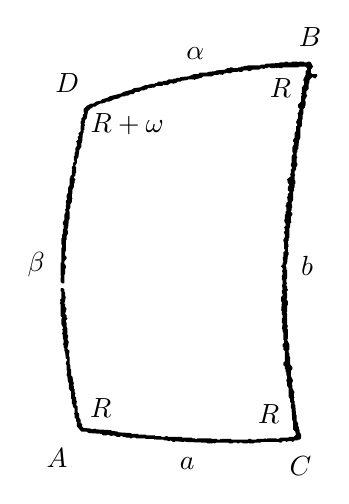
\begin{tikzpicture}[x=0.00939335cm,y=-0.00939335cm]
\fill[even odd rule] (432,74) -- (430,73) -- (428,73) -- (427,74) -- (423,74) -- (422,73) -- (416,73) -- (415,74) -- (413,73) -- (407,73) -- (406,74) -- (401,74) -- (400,73) -- (398,73) -- (397,74) -- (390,74) -- (389,75) -- (371,76) -- (370,77) -- (365,77) -- (364,78) -- (347,78) -- (346,79) -- (342,79) -- (341,80) -- (338,80) -- (337,81) -- (334,81) -- (333,82) -- (327,82) -- (326,81) -- (323,81) -- (322,82) -- (319,82) -- (316,84) -- (304,85) -- (303,86) -- (293,87) -- (292,88) -- (282,88) -- (280,90) -- (274,90) -- (267,93) -- (256,94) -- (255,95) -- (251,95) -- (250,96) -- (247,96) -- (246,97) -- (240,97) -- (237,99) -- (233,99) -- (232,100) -- (226,100) -- (224,102) -- (222,102) -- (221,103) -- (216,103) -- (215,104) -- (213,104) -- (212,105) -- (208,105) -- (201,108) -- (193,109) -- (190,111) -- (179,114) -- (176,116) -- (160,120) -- (157,122) -- (150,124) -- (148,126) -- (142,127) -- (138,130) -- (135,130) -- (129,133) -- (125,137) -- (125,141) -- (126,143) -- (124,145) -- (124,148) -- (122,150) -- (122,153) -- (121,154) -- (121,157) -- (122,158) -- (121,160) -- (121,167) -- (118,170) -- (119,173) -- (117,175) -- (118,178) -- (115,181) -- (116,183) -- (116,187) -- (114,190) -- (114,195) -- (113,196) -- (113,200) -- (112,201) -- (112,206) -- (113,208) -- (111,210) -- (111,213) -- (109,216) -- (109,218) -- (110,219) -- (109,221) -- (109,226) -- (107,228) -- (107,230) -- (106,231) -- (106,240) -- (104,244) -- (104,250) -- (102,254) -- (102,257) -- (103,259) -- (101,261) -- (101,264) -- (102,265) -- (101,267) -- (101,272) -- (100,273) -- (101,276) -- (99,280) -- (99,287) -- (97,290) -- (97,293) -- (98,294) -- (98,299) -- (97,300) -- (97,306) -- (96,307) -- (96,311) -- (95,312) -- (95,320) -- (96,321) -- (96,324) -- (95,325) -- (95,344) -- (94,345) -- (94,362) -- (95,363) -- (94,365) -- (94,371) -- (97,373) -- (99,372) -- (99,361) -- (100,360) -- (100,353) -- (101,352) -- (101,349) -- (99,346) -- (99,343) -- (102,339) -- (102,337) -- (100,335) -- (100,330) -- (101,329) -- (101,315) -- (102,314) -- (102,309) -- (104,305) -- (103,299) -- (104,298) -- (105,287) -- (106,286) -- (106,276) -- (105,274) -- (107,271) -- (107,266) -- (109,263) -- (109,259) -- (110,258) -- (109,256) -- (109,252) -- (110,251) -- (110,246) -- (112,242) -- (112,238) -- (113,237) -- (113,234) -- (114,233) -- (114,232) -- (112,230) -- (112,229) -- (114,227) -- (114,224) -- (115,223) -- (115,216) -- (114,215) -- (114,213) -- (116,210) -- (116,205) -- (118,202) -- (119,193) -- (122,188) -- (122,183) -- (123,182) -- (124,170) -- (125,169) -- (125,166) -- (126,165) -- (126,160) -- (127,159) -- (126,157) -- (127,155) -- (127,152) -- (129,150) -- (131,140) -- (135,136) -- (136,136) -- (138,134) -- (141,134) -- (143,132) -- (147,130) -- (153,129) -- (156,127) -- (160,127) -- (166,124) -- (172,123) -- (177,120) -- (181,120) -- (182,119) -- (185,119) -- (188,117) -- (192,117) -- (195,114) -- (200,114) -- (203,112) -- (207,112) -- (208,111) -- (210,111) -- (212,109) -- (221,108) -- (223,106) -- (231,106) -- (233,104) -- (235,105) -- (238,105) -- (243,102) -- (247,103) -- (248,102) -- (250,102) -- (252,100) -- (256,100) -- (257,99) -- (265,98) -- (266,97) -- (273,97) -- (275,98) -- (276,97) -- (284,95) -- (287,93) -- (298,93) -- (302,91) -- (307,91) -- (308,90) -- (313,91) -- (315,89) -- (317,89) -- (318,88) -- (323,89) -- (327,87) -- (333,87) -- (334,86) -- (336,87) -- (339,87) -- (341,85) -- (347,85) -- (348,86) -- (350,86) -- (353,84) -- (362,84) -- (365,82) -- (369,83) -- (370,82) -- (373,82) -- (374,81) -- (377,81) -- (378,82) -- (383,82) -- (384,81) -- (386,82) -- (388,81) -- (390,82) -- (393,82) -- (394,81) -- (415,81) -- (416,80) -- (425,80) -- (427,82) -- (427,84) -- (425,86) -- (425,91) -- (422,97) -- (422,99) -- (423,100) -- (423,104) -- (420,108) -- (420,115) -- (419,116) -- (420,118) -- (419,120) -- (419,127) -- (415,131) -- (415,135) -- (417,137) -- (417,138) -- (416,139) -- (416,141) -- (414,143) -- (415,145) -- (415,149) -- (412,155) -- (414,159) -- (412,161) -- (412,167) -- (410,170) -- (410,176) -- (408,179) -- (408,181) -- (409,182) -- (409,185) -- (407,189) -- (407,195) -- (408,196) -- (408,198) -- (406,201) -- (406,210) -- (405,211) -- (405,213) -- (407,217) -- (405,219) -- (405,224) -- (404,225) -- (405,228) -- (400,232) -- (401,237) -- (403,239) -- (401,243) -- (401,247) -- (403,249) -- (403,250) -- (401,252) -- (401,255) -- (400,256) -- (401,262) -- (399,264) -- (399,266) -- (398,267) -- (398,269) -- (399,270) -- (399,275) -- (398,276) -- (398,279) -- (397,280) -- (397,286) -- (396,287) -- (397,291) -- (398,292) -- (398,295) -- (396,297) -- (397,299) -- (397,302) -- (396,303) -- (396,305) -- (397,306) -- (397,310) -- (395,314) -- (395,316) -- (396,317) -- (396,326) -- (397,327) -- (397,329) -- (395,331) -- (395,337) -- (394,338) -- (395,344) -- (394,345) -- (394,347) -- (392,349) -- (392,350) -- (394,352) -- (394,355) -- (393,356) -- (394,358) -- (394,361) -- (393,362) -- (393,368) -- (394,369) -- (394,374) -- (393,375) -- (394,381) -- (393,382) -- (393,386) -- (394,387) -- (394,389) -- (392,391) -- (392,397) -- (393,398) -- (392,409) -- (393,410) -- (393,415) -- (394,416) -- (394,419) -- (393,420) -- (393,426) -- (394,427) -- (393,434) -- (394,435) -- (394,438) -- (395,439) -- (395,449) -- (396,450) -- (396,453) -- (394,455) -- (394,458) -- (395,459) -- (395,462) -- (397,464) -- (397,478) -- (395,480) -- (395,483) -- (397,485) -- (397,488) -- (398,489) -- (398,492) -- (399,493) -- (399,497) -- (400,498) -- (400,502) -- (399,503) -- (399,505) -- (400,506) -- (400,511) -- (402,514) -- (402,526) -- (404,529) -- (404,533) -- (406,535) -- (405,537) -- (405,541) -- (406,542) -- (407,558) -- (408,559) -- (408,570) -- (411,573) -- (412,577) -- (409,580) -- (403,580) -- (402,581) -- (392,581) -- (388,583) -- (386,583) -- (385,582) -- (374,582) -- (372,583) -- (370,582) -- (369,583) -- (359,583) -- (358,584) -- (352,584) -- (351,583) -- (348,583) -- (347,584) -- (325,584) -- (324,583) -- (310,583) -- (309,584) -- (306,584) -- (305,583) -- (298,583) -- (297,582) -- (279,582) -- (278,583) -- (276,583) -- (275,582) -- (272,582) -- (271,581) -- (258,581) -- (257,580) -- (239,580) -- (238,579) -- (236,579) -- (235,580) -- (230,580) -- (229,579) -- (222,579) -- (221,578) -- (210,578) -- (209,577) -- (199,577) -- (198,576) -- (190,576) -- (189,575) -- (172,574) -- (171,573) -- (163,572) -- (162,571) -- (142,570) -- (141,569) -- (136,570) -- (135,569) -- (125,568) -- (123,566) -- (123,563) -- (121,561) -- (121,557) -- (119,554) -- (119,549) -- (117,547) -- (117,539) -- (115,537) -- (116,532) -- (115,531) -- (115,527) -- (113,525) -- (114,521) -- (113,520) -- (113,516) -- (112,515) -- (112,512) -- (111,511) -- (112,507) -- (111,506) -- (110,499) -- (108,497) -- (108,489) -- (107,488) -- (107,483) -- (106,482) -- (106,472) -- (105,471) -- (106,464) -- (103,461) -- (105,452) -- (103,448) -- (104,446) -- (104,443) -- (103,442) -- (103,433) -- (102,432) -- (102,426) -- (101,425) -- (101,423) -- (103,421) -- (103,420) -- (102,419) -- (102,416) -- (100,414) -- (102,407) -- (100,404) -- (100,401) -- (99,400) -- (101,391) -- (100,390) -- (100,385) -- (99,384) -- (99,381) -- (97,379) -- (95,379) -- (94,380) -- (94,383) -- (95,384) -- (95,393) -- (93,395) -- (94,397) -- (93,400) -- (94,401) -- (94,417) -- (96,419) -- (95,421) -- (95,428) -- (97,432) -- (97,434) -- (96,435) -- (97,437) -- (96,441) -- (97,442) -- (97,448) -- (98,449) -- (98,453) -- (97,455) -- (98,456) -- (98,459) -- (99,460) -- (99,464) -- (100,465) -- (101,474) -- (103,476) -- (101,480) -- (101,482) -- (102,483) -- (102,490) -- (103,491) -- (102,497) -- (103,498) -- (104,506) -- (105,507) -- (105,515) -- (108,519) -- (108,528) -- (109,529) -- (109,535) -- (110,536) -- (111,540) -- (113,542) -- (113,547) -- (112,549) -- (113,550) -- (113,554) -- (115,556) -- (115,559) -- (116,560) -- (116,566) -- (122,573) -- (129,573) -- (132,575) -- (149,576) -- (151,578) -- (156,578) -- (158,577) -- (162,579) -- (166,578) -- (170,580) -- (174,580) -- (175,579) -- (177,579) -- (178,580) -- (181,580) -- (182,581) -- (187,581) -- (188,582) -- (190,582) -- (191,581) -- (195,581) -- (196,582) -- (208,582) -- (209,583) -- (220,583) -- (221,584) -- (222,583) -- (223,584) -- (233,584) -- (234,585) -- (238,585) -- (239,586) -- (243,585) -- (246,587) -- (248,587) -- (249,586) -- (260,587) -- (262,586) -- (263,587) -- (291,588) -- (292,589) -- (299,589) -- (300,588) -- (302,589) -- (304,588) -- (321,588) -- (322,589) -- (326,589) -- (327,588) -- (332,588) -- (333,589) -- (335,589) -- (336,588) -- (339,588) -- (340,589) -- (346,589) -- (348,588) -- (349,589) -- (355,589) -- (356,588) -- (364,588) -- (365,587) -- (389,587) -- (390,588) -- (392,588) -- (394,586) -- (398,586) -- (399,587) -- (401,586) -- (406,586) -- (408,587) -- (410,585) -- (414,585) -- (415,584) -- (417,584) -- (419,582) -- (419,577) -- (417,574) -- (417,571) -- (416,570) -- (416,567) -- (415,566) -- (415,562) -- (413,559) -- (413,551) -- (412,550) -- (411,537) -- (410,536) -- (410,532) -- (409,531) -- (409,528) -- (410,527) -- (409,525) -- (409,522) -- (410,520) -- (407,514) -- (407,510) -- (406,509) -- (408,504) -- (405,498) -- (405,491) -- (407,489) -- (407,486) -- (404,482) -- (404,472) -- (403,471) -- (403,467) -- (402,466) -- (402,463) -- (403,462) -- (403,455) -- (400,449) -- (401,447) -- (401,435) -- (400,434) -- (401,430) -- (400,429) -- (400,414) -- (399,412) -- (400,411) -- (400,403) -- (401,402) -- (401,397) -- (399,394) -- (400,392) -- (400,386) -- (399,384) -- (401,382) -- (401,381) -- (400,380) -- (400,377) -- (399,376) -- (399,374) -- (400,373) -- (399,371) -- (399,367) -- (400,366) -- (400,355) -- (399,354) -- (399,351) -- (398,349) -- (400,345) -- (401,335) -- (402,334) -- (402,331) -- (401,330) -- (401,324) -- (402,323) -- (401,316) -- (402,315) -- (402,312) -- (403,311) -- (403,298) -- (404,297) -- (404,292) -- (406,290) -- (405,288) -- (405,283) -- (407,280) -- (407,278) -- (405,276) -- (405,275) -- (406,274) -- (406,271) -- (407,270) -- (406,264) -- (408,260) -- (408,249) -- (409,248) -- (409,244) -- (410,243) -- (410,239) -- (411,238) -- (411,234) -- (410,233) -- (410,228) -- (411,226) -- (410,225) -- (410,222) -- (412,219) -- (412,216) -- (414,213) -- (414,211) -- (413,210) -- (413,204) -- (414,203) -- (413,201) -- (413,196) -- (414,195) -- (414,192) -- (415,191) -- (416,180) -- (418,176) -- (418,162) -- (420,160) -- (420,152) -- (421,151) -- (421,145) -- (422,144) -- (422,137) -- (424,135) -- (424,133) -- (425,132) -- (425,127) -- (424,125) -- (427,119) -- (426,117) -- (426,113) -- (429,110) -- (429,103) -- (430,102) -- (430,99) -- (431,97) -- (434,94) -- (438,96) -- (441,92) -- (440,90) -- (434,90) -- (432,88) -- (432,84) -- (435,80) -- cycle;
\node[inner sep=0pt] at (89,609) {$A$};
\node[inner sep=0pt] at (431,40) {$B$};
\node[inner sep=0pt] at (418,620) {$C$};
\node[inner sep=0pt] at (103,102) {$D$};
\node[inner sep=0pt] at (276,62) {$\alpha$};
\node[inner sep=0pt] at (61,347) {$\beta$};
\node[inner sep=0pt] at (265,616) {$a$};
\node[inner sep=0pt] at (427,349) {$b$};
\node[inner sep=0pt] at (148,541) {$R$};
\node[inner sep=0pt] at (375,549) {$R$};
\node[inner sep=0pt] at (391,109) {$R$};
\node[inner sep=0pt] at (184,158) {$R+\omega$};
\end{tikzpicture}
\\[3pt]Fig. 1.\end{minipage}\end{center}

Es ist aber, wie die Figur 2 zeigt,
\[
\lambda = F(\rho, \rho) = CR,
\]
also
\[
F(a,b) = \frac{\lambda}{R}\cdot\omega.]
\]

Man hat [daher]:
\[
\tag*{1)} \omega = \frac{R}{\lambda} F(a,b).
\]

\begin{center}\begin{minipage}{\linewidth}\centering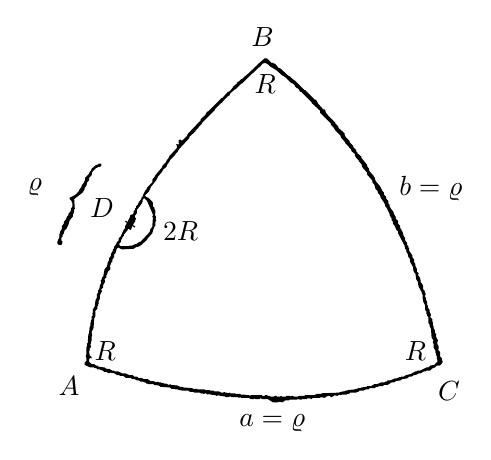
\begin{tikzpicture}[x=0.00819892cm,y=-0.00819892cm]
\fill[even odd rule] (141,232) -- (138,232) -- (136,234) -- (134,234) -- (127,240) -- (126,243) -- (124,245) -- (122,249) -- (117,254) -- (117,257) -- (114,263) -- (112,265) -- (111,269) -- (109,271) -- (107,275) -- (101,281) -- (93,285) -- (93,287) -- (96,290) -- (96,292) -- (97,293) -- (97,299) -- (95,302) -- (95,305) -- (91,310) -- (91,312) -- (89,314) -- (87,319) -- (84,322) -- (84,325) -- (81,329) -- (81,333) -- (78,338) -- (78,340) -- (77,341) -- (77,346) -- (74,353) -- (74,356) -- (76,358) -- (80,358) -- (81,357) -- (82,353) -- (80,351) -- (80,347) -- (82,345) -- (82,343) -- (84,340) -- (85,336) -- (88,333) -- (91,327) -- (93,320) -- (98,314) -- (98,311) -- (99,310) -- (99,308) -- (100,307) -- (100,303) -- (101,302) -- (100,287) -- (113,277) -- (116,272) -- (116,270) -- (119,266) -- (120,261) -- (123,258) -- (123,255) -- (124,253) -- (127,250) -- (128,245) -- (134,239) -- (138,237) -- (140,237) -- (142,235) -- (142,233) -- cycle
(671,538) -- (670,537) -- (670,534) -- (667,531) -- (667,524) -- (664,521) -- (665,519) -- (665,515) -- (663,512) -- (663,508) -- (664,506) -- (661,501) -- (661,496) -- (659,494) -- (659,490) -- (657,487) -- (657,484) -- (656,483) -- (656,478) -- (655,477) -- (655,473) -- (652,470) -- (653,466) -- (651,462) -- (651,459) -- (648,455) -- (648,452) -- (647,451) -- (647,446) -- (645,443) -- (645,440) -- (644,439) -- (644,436) -- (645,434) -- (644,433) -- (643,429) -- (641,427) -- (641,422) -- (639,418) -- (637,416) -- (637,412) -- (636,411) -- (636,409) -- (633,405) -- (634,402) -- (631,399) -- (631,395) -- (629,391) -- (629,388) -- (627,385) -- (627,381) -- (624,377) -- (624,374) -- (619,367) -- (619,363) -- (618,362) -- (618,360) -- (616,358) -- (616,355) -- (613,351) -- (613,347) -- (611,345) -- (609,338) -- (605,331) -- (605,328) -- (602,325) -- (602,321) -- (599,318) -- (598,314) -- (595,309) -- (595,307) -- (591,302) -- (589,298) -- (589,296) -- (587,294) -- (587,290) -- (584,287) -- (583,283) -- (580,280) -- (580,277) -- (578,275) -- (574,267) -- (568,260) -- (566,256) -- (566,254) -- (564,252) -- (564,251) -- (557,243) -- (557,240) -- (554,236) -- (554,234) -- (545,223) -- (545,221) -- (539,216) -- (539,215) -- (537,213) -- (537,211) -- (533,207) -- (532,204) -- (527,199) -- (527,197) -- (521,191) -- (519,187) -- (519,185) -- (510,177) -- (509,174) -- (505,170) -- (505,169) -- (493,157) -- (493,156) -- (490,153) -- (489,149) -- (488,148) -- (486,148) -- (478,139) -- (476,135) -- (474,133) -- (473,133) -- (458,118) -- (457,118) -- (442,103) -- (441,103) -- (433,96) -- (432,96) -- (419,84) -- (417,84) -- (412,78) -- (408,76) -- (406,76) -- (399,69) -- (395,69) -- (386,77) -- (385,77) -- (384,79) -- (366,96) -- (365,96) -- (360,101) -- (359,101) -- (355,105) -- (354,105) -- (352,107) -- (352,108) -- (346,113) -- (346,114) -- (341,120) -- (338,121) -- (330,130) -- (329,130) -- (308,151) -- (307,151) -- (305,153) -- (303,157) -- (296,163) -- (296,165) -- (276,186) -- (275,189) -- (268,196) -- (266,196) -- (265,195) -- (263,195) -- (262,196) -- (262,200) -- (263,201) -- (261,203) -- (260,202) -- (258,202) -- (259,204) -- (259,208) -- (247,221) -- (246,224) -- (244,226) -- (242,230) -- (237,235) -- (236,238) -- (225,251) -- (225,252) -- (221,257) -- (221,261) -- (213,269) -- (212,272) -- (210,274) -- (207,280) -- (207,282) -- (204,285) -- (204,287) -- (200,292) -- (199,295) -- (196,298) -- (196,300) -- (194,302) -- (194,304) -- (192,306) -- (192,309) -- (190,311) -- (188,311) -- (187,312) -- (186,316) -- (179,329) -- (179,332) -- (177,334) -- (172,345) -- (169,348) -- (169,351) -- (166,354) -- (165,357) -- (162,361) -- (162,363) -- (160,365) -- (160,367) -- (157,372) -- (157,375) -- (154,379) -- (154,382) -- (152,385) -- (151,391) -- (147,396) -- (145,407) -- (143,409) -- (143,411) -- (141,413) -- (142,417) -- (140,420) -- (139,426) -- (137,429) -- (137,432) -- (135,435) -- (135,440) -- (133,444) -- (132,453) -- (129,458) -- (129,463) -- (128,464) -- (129,467) -- (127,469) -- (127,474) -- (126,475) -- (126,478) -- (125,479) -- (125,484) -- (124,485) -- (123,495) -- (122,496) -- (121,510) -- (120,511) -- (120,515) -- (119,516) -- (119,528) -- (118,529) -- (118,532) -- (119,533) -- (119,538) -- (116,541) -- (116,544) -- (125,548) -- (131,548) -- (132,549) -- (134,549) -- (136,551) -- (140,551) -- (141,552) -- (143,552) -- (147,555) -- (150,555) -- (154,557) -- (156,556) -- (162,557) -- (167,560) -- (170,560) -- (171,561) -- (176,561) -- (180,564) -- (187,564) -- (190,566) -- (194,566) -- (197,568) -- (200,568) -- (203,570) -- (207,570) -- (208,571) -- (210,571) -- (212,573) -- (214,573) -- (215,574) -- (223,574) -- (224,575) -- (231,576) -- (234,578) -- (248,579) -- (251,581) -- (256,581) -- (257,582) -- (261,582) -- (262,583) -- (266,583) -- (267,584) -- (277,584) -- (280,586) -- (285,586) -- (286,587) -- (295,587) -- (296,588) -- (299,588) -- (300,589) -- (304,588) -- (307,590) -- (310,589) -- (311,590) -- (319,591) -- (320,592) -- (325,591) -- (326,592) -- (334,593) -- (335,594) -- (339,594) -- (340,593) -- (343,593) -- (344,594) -- (354,594) -- (355,595) -- (358,594) -- (359,595) -- (370,595) -- (374,597) -- (378,597) -- (379,596) -- (381,597) -- (387,597) -- (388,596) -- (390,596) -- (391,597) -- (400,597) -- (408,602) -- (416,602) -- (417,601) -- (423,602) -- (427,599) -- (433,599) -- (434,598) -- (445,598) -- (446,597) -- (452,598) -- (453,597) -- (460,597) -- (461,596) -- (466,596) -- (468,597) -- (470,595) -- (481,595) -- (482,594) -- (488,595) -- (493,592) -- (496,592) -- (498,594) -- (499,594) -- (504,591) -- (508,592) -- (511,590) -- (513,591) -- (515,590) -- (522,590) -- (523,589) -- (526,589) -- (528,587) -- (537,587) -- (538,586) -- (540,586) -- (542,584) -- (548,584) -- (552,582) -- (556,582) -- (558,580) -- (566,580) -- (568,578) -- (571,578) -- (572,577) -- (578,577) -- (580,575) -- (586,575) -- (592,571) -- (596,571) -- (599,569) -- (606,568) -- (608,566) -- (616,565) -- (619,562) -- (623,562) -- (626,560) -- (631,559) -- (634,557) -- (637,557) -- (642,554) -- (645,554) -- (646,553) -- (651,553) -- (656,549) -- (659,548) -- (662,545) -- (666,545) -- (668,544) -- (671,540) -- cycle
(209,286) -- (213,290) -- (222,311) -- (222,313) -- (221,314) -- (222,316) -- (221,330) -- (218,334) -- (217,338) -- (203,353) -- (200,354) -- (196,357) -- (194,357) -- (190,359) -- (186,359) -- (185,360) -- (172,360) -- (170,358) -- (170,356) -- (172,354) -- (173,350) -- (175,346) -- (177,344) -- (177,342) -- (183,335) -- (183,334) -- (184,333) -- (186,333) -- (187,335) -- (188,334) -- (196,317) -- (194,315) -- (194,313) -- (197,309) -- (197,304) -- (204,295) -- (206,291) -- (206,288) -- (208,286) -- cycle
(392,77) -- (396,76) -- (400,78) -- (403,81) -- (413,87) -- (422,95) -- (427,98) -- (435,106) -- (439,108) -- (442,111) -- (442,112) -- (445,115) -- (446,115) -- (449,118) -- (449,119) -- (451,121) -- (452,121) -- (468,137) -- (468,138) -- (481,150) -- (481,153) -- (498,170) -- (498,172) -- (502,176) -- (505,181) -- (513,189) -- (513,191) -- (520,199) -- (520,200) -- (526,206) -- (526,207) -- (529,210) -- (530,213) -- (535,217) -- (535,219) -- (537,223) -- (541,227) -- (541,228) -- (546,234) -- (546,237) -- (554,246) -- (554,249) -- (562,258) -- (562,261) -- (565,264) -- (567,271) -- (570,274) -- (571,278) -- (574,281) -- (575,285) -- (580,292) -- (582,296) -- (582,298) -- (584,300) -- (589,310) -- (589,312) -- (592,317) -- (592,320) -- (594,322) -- (594,325) -- (597,329) -- (599,334) -- (602,337) -- (602,340) -- (612,359) -- (612,361) -- (613,362) -- (613,364) -- (615,366) -- (615,369) -- (617,372) -- (618,377) -- (620,379) -- (621,385) -- (625,392) -- (626,399) -- (629,403) -- (630,411) -- (633,416) -- (633,420) -- (634,421) -- (634,423) -- (639,432) -- (639,434) -- (640,435) -- (640,442) -- (641,443) -- (641,446) -- (644,452) -- (644,459) -- (646,461) -- (646,465) -- (647,466) -- (647,468) -- (649,470) -- (649,479) -- (651,482) -- (651,484) -- (653,488) -- (654,502) -- (657,506) -- (656,508) -- (656,510) -- (657,511) -- (657,517) -- (660,522) -- (660,525) -- (661,526) -- (661,529) -- (662,530) -- (662,535) -- (663,536) -- (663,539) -- (658,544) -- (652,545) -- (649,548) -- (646,548) -- (636,553) -- (632,553) -- (631,554) -- (629,554) -- (622,558) -- (614,560) -- (611,562) -- (607,562) -- (606,563) -- (604,563) -- (600,565) -- (597,565) -- (590,568) -- (586,568) -- (584,570) -- (582,570) -- (581,571) -- (576,571) -- (569,574) -- (565,574) -- (560,577) -- (554,577) -- (553,578) -- (545,579) -- (544,580) -- (540,580) -- (539,581) -- (536,581) -- (535,582) -- (524,583) -- (523,584) -- (520,584) -- (519,585) -- (516,585) -- (515,586) -- (512,586) -- (511,587) -- (484,588) -- (483,589) -- (476,589) -- (472,591) -- (458,591) -- (457,592) -- (448,592) -- (447,593) -- (440,593) -- (439,592) -- (437,592) -- (436,593) -- (434,592) -- (429,592) -- (428,593) -- (422,593) -- (421,592) -- (419,593) -- (414,593) -- (413,592) -- (411,592) -- (410,593) -- (404,593) -- (403,592) -- (400,592) -- (399,591) -- (396,591) -- (395,592) -- (392,592) -- (391,591) -- (374,591) -- (372,592) -- (371,591) -- (366,591) -- (365,590) -- (358,590) -- (357,589) -- (350,589) -- (349,588) -- (342,588) -- (341,587) -- (338,588) -- (337,587) -- (334,587) -- (333,586) -- (331,587) -- (328,587) -- (324,585) -- (317,585) -- (316,584) -- (311,584) -- (310,583) -- (303,583) -- (302,582) -- (291,582) -- (290,581) -- (284,581) -- (283,580) -- (269,579) -- (268,578) -- (264,578) -- (260,576) -- (250,575) -- (249,574) -- (246,575) -- (243,573) -- (239,573) -- (238,572) -- (235,572) -- (234,571) -- (231,571) -- (230,570) -- (226,571) -- (223,569) -- (218,569) -- (214,566) -- (208,566) -- (204,564) -- (199,564) -- (197,562) -- (193,562) -- (191,560) -- (186,560) -- (179,557) -- (174,557) -- (168,554) -- (163,554) -- (162,553) -- (159,553) -- (154,550) -- (150,550) -- (147,548) -- (138,547) -- (136,545) -- (134,545) -- (131,543) -- (128,543) -- (126,542) -- (123,539) -- (123,535) -- (125,533) -- (127,534) -- (127,532) -- (124,529) -- (123,523) -- (124,522) -- (124,519) -- (126,516) -- (125,512) -- (126,511) -- (126,508) -- (127,507) -- (127,500) -- (128,499) -- (127,493) -- (130,487) -- (131,472) -- (133,468) -- (133,460) -- (136,457) -- (136,453) -- (137,452) -- (137,450) -- (138,449) -- (138,445) -- (140,441) -- (140,436) -- (143,430) -- (142,427) -- (145,424) -- (145,420) -- (148,415) -- (147,411) -- (150,408) -- (150,405) -- (151,404) -- (152,400) -- (156,396) -- (156,393) -- (155,391) -- (156,390) -- (157,386) -- (159,384) -- (159,381) -- (162,377) -- (162,373) -- (164,371) -- (166,364) -- (168,362) -- (174,365) -- (192,364) -- (197,361) -- (199,361) -- (203,359) -- (213,350) -- (213,349) -- (221,340) -- (223,333) -- (224,332) -- (224,330) -- (226,328) -- (226,322) -- (227,321) -- (227,319) -- (226,318) -- (227,315) -- (225,311) -- (226,309) -- (226,305) -- (225,304) -- (224,300) -- (222,298) -- (222,293) -- (221,291) -- (215,285) -- (212,284) -- (210,282) -- (210,281) -- (216,275) -- (219,268) -- (227,258) -- (230,252) -- (236,245) -- (238,241) -- (243,237) -- (245,232) -- (247,230) -- (249,226) -- (257,218) -- (257,217) -- (260,214) -- (263,209) -- (278,193) -- (279,190) -- (288,182) -- (288,181) -- (293,176) -- (293,175) -- (298,170) -- (298,169) -- (318,149) -- (318,148) -- (328,138) -- (329,138) -- (330,136) -- (339,127) -- (341,126) -- (342,123) -- (349,117) -- (350,117) -- (359,108) -- (360,108) -- (376,92) -- (377,92) -- (386,83) -- (387,83) -- cycle;
\node[inner sep=0pt] at (92,577) {$A$};
\node[inner sep=0pt] at (392,36) {$B$};
\node[inner sep=0pt] at (681,584) {$C$};
\node[inner sep=0pt] at (143,301) {$D$};
\node[inner sep=0pt] at (39,268) {$\varrho$};
\node[inner sep=0pt] at (653,271) {$b=\varrho$};
\node[inner sep=0pt] at (407,635) {$a=\varrho$};
\node[inner sep=0pt] at (396,108) {$R$};
\node[inner sep=0pt] at (148,523) {$R$};
\node[inner sep=0pt] at (629,522) {$R$};
\node[inner sep=0pt] at (265,337) {$2R$};
\node[inner sep=0pt] at (187,327) {$\ast$};
\end{tikzpicture}
\\[3pt]Fig. 2.\end{minipage}\end{center}

\Needspace{28\baselineskip}
[Wendet man diese Gleichung auf das Viereck $ACFE$ an (Fig. 3), so wird

\begin{center}\begin{minipage}{\linewidth}\centering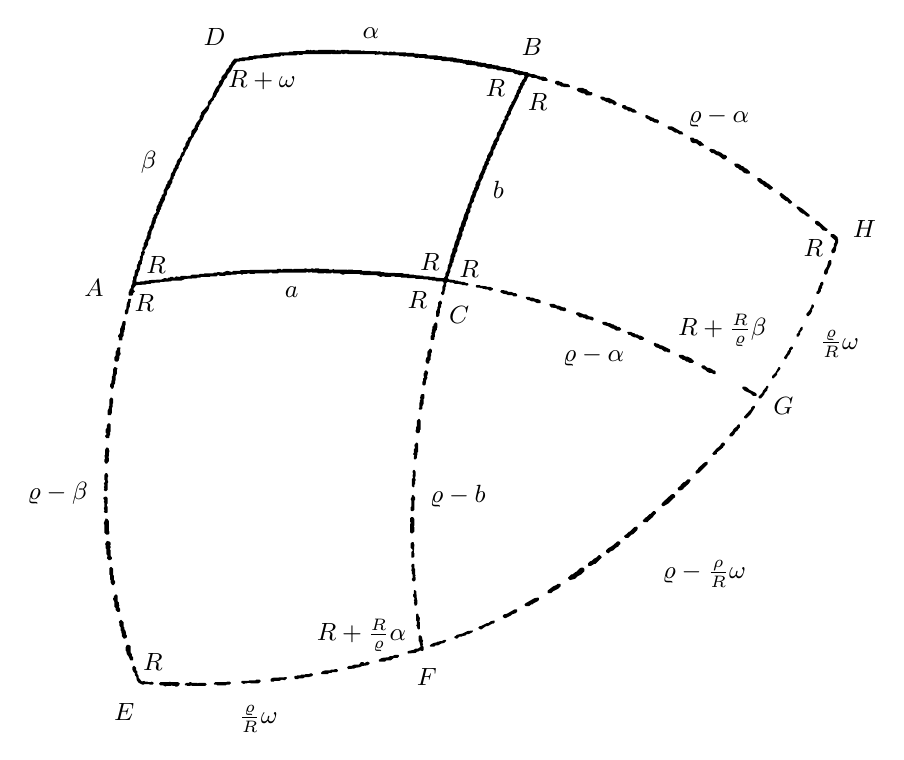
\begin{tikzpicture}[x=0.00790378cm,y=-0.00790378cm]
\fill[even odd rule] (292,1078) -- (293,1080) -- (295,1080) -- (296,1081) -- (301,1081) -- (302,1080) -- (304,1081) -- (325,1081) -- (327,1079) -- (327,1078) -- (325,1076) -- (315,1076) -- (313,1077) -- (312,1076) -- (303,1076) -- (302,1075) -- (300,1075) -- (299,1076) -- (295,1076) -- cycle
(366,1076) -- (364,1074) -- (360,1074) -- (359,1075) -- (341,1075) -- (339,1077) -- (339,1078) -- (340,1079) -- (343,1079) -- (344,1080) -- (358,1080) -- (359,1079) -- (364,1079) -- (366,1077) -- cycle
(284,1077) -- (281,1075) -- (270,1075) -- (268,1074) -- (267,1075) -- (253,1075) -- (251,1077) -- (251,1078) -- (253,1080) -- (257,1080) -- (261,1082) -- (263,1081) -- (270,1081) -- (271,1080) -- (273,1081) -- (276,1081) -- (277,1082) -- (280,1082) -- (283,1080) -- cycle
(414,1073) -- (412,1071) -- (407,1071) -- (406,1072) -- (396,1072) -- (395,1073) -- (384,1073) -- (383,1074) -- (383,1076) -- (387,1078) -- (389,1077) -- (392,1077) -- (393,1076) -- (397,1076) -- (398,1077) -- (410,1077) -- (412,1076) -- (414,1074) -- cycle
(456,1068) -- (455,1067) -- (433,1068) -- (430,1070) -- (430,1073) -- (431,1074) -- (435,1074) -- (436,1073) -- (444,1073) -- (448,1071) -- (453,1072) -- (456,1069) -- cycle
(498,1063) -- (496,1061) -- (493,1061) -- (492,1062) -- (486,1062) -- (485,1063) -- (479,1063) -- (478,1064) -- (473,1064) -- (472,1065) -- (469,1065) -- (468,1066) -- (468,1068) -- (470,1070) -- (474,1070) -- (475,1069) -- (482,1069) -- (485,1067) -- (492,1067) -- (493,1066) -- (495,1066) -- (497,1065) -- cycle
(538,1056) -- (536,1054) -- (533,1054) -- (532,1055) -- (527,1055) -- (526,1056) -- (517,1056) -- (516,1057) -- (514,1057) -- (511,1060) -- (511,1061) -- (512,1062) -- (522,1062) -- (524,1060) -- (528,1060) -- (529,1059) -- (536,1059) -- (538,1057) -- cycle
(208,1051) -- (208,1055) -- (210,1059) -- (212,1061) -- (212,1064) -- (214,1066) -- (215,1072) -- (218,1076) -- (224,1079) -- (226,1079) -- (227,1078) -- (235,1078) -- (236,1079) -- (240,1079) -- (242,1077) -- (242,1076) -- (239,1074) -- (237,1075) -- (233,1075) -- (232,1074) -- (228,1074) -- (227,1073) -- (223,1074) -- (218,1068) -- (218,1065) -- (216,1062) -- (216,1058) -- (214,1056) -- (214,1052) -- (211,1049) -- (210,1049) -- cycle
(589,1044) -- (586,1042) -- (583,1043) -- (581,1045) -- (579,1043) -- (575,1043) -- (572,1047) -- (564,1047) -- (560,1049) -- (556,1049) -- (554,1050) -- (553,1052) -- (555,1054) -- (565,1053) -- (566,1052) -- (573,1051) -- (577,1049) -- (585,1048) -- (587,1047) -- (589,1045) -- cycle
(636,1032) -- (635,1031) -- (630,1031) -- (626,1033) -- (622,1033) -- (619,1035) -- (609,1036) -- (604,1039) -- (604,1041) -- (605,1042) -- (614,1042) -- (616,1040) -- (623,1040) -- (628,1036) -- (634,1036) -- (636,1034) -- cycle
(199,1015) -- (197,1019) -- (197,1024) -- (198,1025) -- (199,1030) -- (202,1034) -- (204,1039) -- (205,1040) -- (208,1040) -- (209,1039) -- (209,1035) -- (207,1033) -- (207,1030) -- (205,1027) -- (205,1017) -- (202,1015) -- cycle
(712,1008) -- (711,1007) -- (709,1007) -- (705,1009) -- (702,1009) -- (701,1010) -- (698,1010) -- (697,1011) -- (692,1012) -- (688,1014) -- (686,1016) -- (686,1017) -- (687,1018) -- (693,1018) -- (695,1016) -- (699,1016) -- (704,1013) -- (709,1012) -- (712,1009) -- cycle
(671,1000) -- (669,1000) -- (668,1001) -- (668,1009) -- (669,1010) -- (671,1018) -- (667,1021) -- (663,1021) -- (660,1023) -- (651,1025) -- (650,1026) -- (650,1028) -- (651,1029) -- (663,1028) -- (665,1026) -- (667,1026) -- (670,1024) -- (674,1025) -- (676,1023) -- (676,1019) -- (674,1016) -- (675,1014) -- (674,1012) -- (675,1008) -- (674,1007) -- (673,1002) -- cycle
(755,993) -- (754,992) -- (746,993) -- (738,997) -- (729,999) -- (727,1001) -- (726,1001) -- (725,1003) -- (728,1005) -- (730,1005) -- (733,1002) -- (737,1002) -- (738,1001) -- (743,1000) -- (745,998) -- (748,998) -- (754,995) -- cycle
(790,977) -- (789,976) -- (784,977) -- (780,980) -- (778,980) -- (768,985) -- (766,985) -- (764,987) -- (764,988) -- (767,990) -- (769,990) -- (776,985) -- (779,985) -- (786,981) -- (788,981) -- (790,979) -- cycle
(189,975) -- (186,978) -- (187,980) -- (187,984) -- (189,987) -- (189,992) -- (190,993) -- (190,996) -- (191,997) -- (191,1001) -- (194,1005) -- (196,1005) -- (199,1003) -- (199,1000) -- (198,999) -- (197,993) -- (195,990) -- (195,987) -- (194,986) -- (194,979) -- (190,975) -- cycle
(665,965) -- (664,966) -- (664,976) -- (665,977) -- (665,982) -- (664,984) -- (665,985) -- (666,989) -- (667,990) -- (669,990) -- (670,989) -- (670,979) -- (669,978) -- (670,972) -- (668,969) -- (668,967) -- (666,965) -- cycle
(826,959) -- (825,958) -- (822,958) -- (810,965) -- (805,966) -- (803,968) -- (803,970) -- (806,972) -- (808,972) -- (816,968) -- (818,966) -- (824,964) -- (826,962) -- cycle
(861,940) -- (860,939) -- (854,940) -- (840,948) -- (838,950) -- (838,951) -- (840,953) -- (845,953) -- (849,950) -- (851,950) -- (853,948) -- (859,945) -- (861,943) -- cycle
(181,934) -- (178,937) -- (178,939) -- (177,940) -- (177,942) -- (179,946) -- (179,954) -- (181,956) -- (181,959) -- (184,962) -- (187,962) -- (188,961) -- (188,957) -- (186,954) -- (187,952) -- (186,950) -- (186,947) -- (184,945) -- (184,936) -- (182,934) -- cycle
(661,927) -- (660,928) -- (660,933) -- (659,934) -- (659,937) -- (661,940) -- (661,942) -- (660,943) -- (661,946) -- (660,948) -- (661,949) -- (661,951) -- (662,952) -- (664,952) -- (666,949) -- (666,943) -- (665,942) -- (664,929) -- (662,927) -- cycle
(896,918) -- (895,917) -- (891,917) -- (889,919) -- (884,921) -- (875,928) -- (875,931) -- (876,932) -- (881,932) -- (884,929) -- (892,925) -- (896,921) -- cycle
(934,893) -- (932,891) -- (929,891) -- (927,892) -- (921,898) -- (920,898) -- (915,902) -- (913,902) -- (908,907) -- (908,908) -- (911,911) -- (919,909) -- (923,905) -- (929,902) -- (934,897) -- cycle
(173,890) -- (171,892) -- (171,902) -- (172,903) -- (172,910) -- (173,911) -- (173,915) -- (174,917) -- (176,919) -- (178,919) -- (180,916) -- (180,913) -- (178,910) -- (178,904) -- (177,903) -- (177,893) -- (174,890) -- cycle
(658,885) -- (656,887) -- (656,890) -- (657,891) -- (656,896) -- (657,897) -- (657,901) -- (658,902) -- (658,908) -- (657,909) -- (657,911) -- (659,913) -- (661,913) -- (663,911) -- (663,907) -- (662,906) -- (663,904) -- (662,902) -- (662,893) -- (661,892) -- (661,886) -- (660,885) -- cycle
(962,874) -- (959,871) -- (957,871) -- (953,875) -- (949,877) -- (946,880) -- (943,881) -- (940,884) -- (940,887) -- (941,888) -- (945,888) -- (950,885) -- (952,885) -- (962,875) -- cycle
(657,850) -- (655,852) -- (655,859) -- (658,862) -- (658,864) -- (656,866) -- (656,874) -- (657,875) -- (659,875) -- (661,873) -- (661,868) -- (660,867) -- (661,854) -- (660,853) -- (660,851) -- (659,850) -- cycle
(992,851) -- (990,849) -- (987,849) -- (979,856) -- (972,860) -- (969,863) -- (969,866) -- (973,868) -- (976,865) -- (981,863) -- (985,859) -- (989,857) -- (989,856) -- (992,853) -- cycle
(167,848) -- (164,853) -- (165,855) -- (165,860) -- (166,861) -- (166,869) -- (168,872) -- (167,876) -- (170,879) -- (172,879) -- (175,877) -- (175,875) -- (173,872) -- (173,863) -- (172,862) -- (172,860) -- (173,859) -- (173,857) -- (172,856) -- (173,854) -- (173,851) -- (171,849) -- cycle
(1020,827) -- (1018,825) -- (1014,826) -- (1007,833) -- (1006,833) -- (1001,838) -- (1000,838) -- (998,840) -- (998,841) -- (1000,843) -- (1005,843) -- (1010,838) -- (1013,837) -- (1019,831) -- cycle
(165,812) -- (162,819) -- (162,821) -- (163,822) -- (163,835) -- (166,838) -- (169,838) -- (171,836) -- (171,833) -- (170,832) -- (170,816) -- (168,813) -- cycle
(656,810) -- (654,812) -- (654,817) -- (655,818) -- (655,820) -- (654,821) -- (654,834) -- (656,836) -- (658,836) -- (661,833) -- (661,826) -- (660,825) -- (661,823) -- (661,813) -- (659,810) -- cycle
(1049,802) -- (1047,800) -- (1045,800) -- (1040,805) -- (1039,805) -- (1034,810) -- (1033,810) -- (1028,815) -- (1028,816) -- (1030,818) -- (1036,818) -- (1037,816) -- (1045,809) -- (1045,808) -- (1049,804) -- cycle
(164,777) -- (161,779) -- (163,783) -- (162,785) -- (163,787) -- (163,794) -- (162,795) -- (163,799) -- (162,801) -- (164,803) -- (167,803) -- (168,802) -- (168,793) -- (167,792) -- (167,789) -- (168,788) -- (168,779) -- (166,777) -- cycle
(659,774) -- (657,775) -- (657,777) -- (655,781) -- (656,783) -- (656,793) -- (655,794) -- (655,799) -- (656,800) -- (659,800) -- (661,798) -- (661,783) -- (662,782) -- (662,778) -- cycle
(1080,775) -- (1078,773) -- (1075,773) -- (1073,774) -- (1059,787) -- (1058,790) -- (1060,792) -- (1062,792) -- (1069,788) -- (1078,779) -- (1080,778) -- cycle
(1105,751) -- (1103,749) -- (1100,749) -- (1096,753) -- (1093,754) -- (1089,758) -- (1089,759) -- (1084,763) -- (1085,766) -- (1086,767) -- (1089,767) -- (1093,765) -- (1094,763) -- (1102,756) -- cycle
(167,739) -- (165,739) -- (163,742) -- (163,750) -- (164,751) -- (164,753) -- (162,756) -- (163,758) -- (163,760) -- (162,761) -- (163,764) -- (162,766) -- (164,768) -- (166,768) -- (168,766) -- (168,755) -- (169,754) -- (169,752) -- (168,751) -- (168,746) -- (169,745) -- (169,743) -- cycle
(661,734) -- (660,734) -- (658,736) -- (658,738) -- (659,739) -- (658,744) -- (659,746) -- (657,749) -- (657,760) -- (659,762) -- (661,761) -- (661,758) -- (662,757) -- (662,752) -- (663,751) -- (663,749) -- (662,748) -- (662,745) -- (663,744) -- (663,737) -- cycle
(1131,721) -- (1127,722) -- (1117,731) -- (1117,732) -- (1113,736) -- (1113,739) -- (1114,740) -- (1118,739) -- (1132,725) -- (1132,722) -- cycle
(168,698) -- (166,698) -- (164,702) -- (164,710) -- (163,711) -- (164,716) -- (163,717) -- (163,721) -- (165,724) -- (167,724) -- (170,720) -- (170,715) -- (169,713) -- (170,712) -- (170,706) -- (171,705) -- (171,703) -- (170,702) -- (170,700) -- cycle
(1158,690) -- (1156,690) -- (1153,693) -- (1153,694) -- (1149,698) -- (1148,698) -- (1140,707) -- (1140,708) -- (1142,710) -- (1146,709) -- (1147,708) -- (1147,706) -- (1157,698) -- (1157,697) -- (1160,694) -- (1160,692) -- cycle
(665,690) -- (664,690) -- (661,694) -- (662,699) -- (660,701) -- (660,707) -- (659,708) -- (659,709) -- (661,711) -- (660,713) -- (660,716) -- (661,717) -- (663,717) -- (665,715) -- (665,711) -- (666,710) -- (666,706) -- (667,705) -- (667,692) -- cycle
(1183,661) -- (1181,661) -- (1179,663) -- (1179,664) -- (1174,668) -- (1172,672) -- (1168,676) -- (1167,678) -- (1168,680) -- (1172,680) -- (1175,677) -- (1177,673) -- (1181,670) -- (1181,669) -- (1184,666) -- (1184,662) -- cycle
(171,659) -- (169,659) -- (167,662) -- (167,666) -- (165,669) -- (165,674) -- (166,675) -- (166,677) -- (164,679) -- (164,680) -- (166,683) -- (170,683) -- (171,682) -- (171,679) -- (172,678) -- (172,673) -- (173,672) -- (173,661) -- cycle
(669,652) -- (668,652) -- (665,655) -- (665,664) -- (664,665) -- (664,669) -- (663,670) -- (663,672) -- (665,675) -- (668,675) -- (670,673) -- (670,670) -- (671,669) -- (671,655) -- cycle
(1207,631) -- (1205,631) -- (1202,634) -- (1202,636) -- (1191,648) -- (1191,650) -- (1192,651) -- (1195,651) -- (1201,645) -- (1208,634) -- (1208,632) -- cycle
(175,618) -- (173,618) -- (171,621) -- (171,631) -- (170,632) -- (170,635) -- (168,639) -- (168,645) -- (169,646) -- (173,646) -- (175,642) -- (175,634) -- (176,633) -- (176,628) -- (177,627) -- (177,620) -- cycle
(676,612) -- (673,612) -- (671,614) -- (671,616) -- (670,617) -- (671,621) -- (670,622) -- (670,625) -- (669,626) -- (669,634) -- (668,635) -- (669,637) -- (672,637) -- (674,635) -- (674,631) -- (676,627) -- (676,620) -- (677,619) -- (677,613) -- cycle
(1188,601) -- (1188,603) -- (1192,607) -- (1201,611) -- (1205,615) -- (1210,615) -- (1211,614) -- (1211,612) -- (1209,610) -- (1199,605) -- (1196,602) -- (1192,600) -- (1189,600) -- cycle
(1229,599) -- (1227,599) -- (1226,600) -- (1226,601) -- (1221,607) -- (1220,610) -- (1214,616) -- (1214,618) -- (1215,619) -- (1218,619) -- (1223,613) -- (1224,610) -- (1228,606) -- (1228,604) -- (1230,601) -- cycle
(680,574) -- (679,574) -- (677,576) -- (677,578) -- (676,579) -- (676,583) -- (677,585) -- (675,587) -- (675,591) -- (674,592) -- (674,597) -- (675,598) -- (678,598) -- (679,597) -- (680,590) -- (682,586) -- (681,583) -- (682,582) -- (683,577) -- cycle
(1248,569) -- (1246,569) -- (1241,578) -- (1236,583) -- (1236,586) -- (1237,587) -- (1238,587) -- (1244,581) -- (1244,578) -- (1249,572) -- (1249,570) -- cycle
(181,569) -- (179,569) -- (177,572) -- (177,579) -- (176,580) -- (176,583) -- (175,584) -- (175,590) -- (174,591) -- (174,594) -- (172,597) -- (172,600) -- (175,604) -- (177,603) -- (178,601) -- (178,598) -- (180,595) -- (180,591) -- (181,590) -- (181,583) -- (183,579) -- (183,573) -- (184,571) -- cycle
(1122,568) -- (1122,569) -- (1125,572) -- (1128,573) -- (1131,576) -- (1135,578) -- (1138,578) -- (1142,580) -- (1144,580) -- (1145,579) -- (1145,576) -- (1143,574) -- (1141,574) -- (1139,572) -- (1135,570) -- (1132,570) -- (1127,566) -- (1124,566) -- cycle
(1086,550) -- (1086,552) -- (1089,555) -- (1090,555) -- (1092,557) -- (1096,558) -- (1098,560) -- (1100,560) -- (1103,562) -- (1108,562) -- (1110,560) -- (1110,559) -- (1106,555) -- (1100,552) -- (1097,552) -- (1092,549) -- (1087,549) -- cycle
(687,539) -- (686,539) -- (682,544) -- (682,552) -- (680,554) -- (680,556) -- (679,557) -- (679,560) -- (681,563) -- (684,563) -- (685,562) -- (685,559) -- (687,557) -- (687,552) -- (688,551) -- (688,546) -- (689,545) -- (689,541) -- cycle
(188,537) -- (185,537) -- (183,539) -- (183,541) -- (181,544) -- (181,550) -- (179,553) -- (179,558) -- (181,560) -- (184,560) -- (186,558) -- (186,556) -- (187,555) -- (187,551) -- (189,548) -- (189,546) -- (188,545) -- (188,540) -- (189,538) -- cycle
(1268,536) -- (1266,536) -- (1263,539) -- (1263,541) -- (1261,543) -- (1260,546) -- (1255,553) -- (1255,554) -- (1257,556) -- (1258,556) -- (1260,554) -- (1261,551) -- (1264,548) -- (1266,544) -- (1266,542) -- (1269,539) -- (1269,537) -- cycle
(1046,531) -- (1046,534) -- (1049,537) -- (1053,538) -- (1056,540) -- (1058,540) -- (1063,544) -- (1067,544) -- (1068,545) -- (1071,545) -- (1072,544) -- (1072,541) -- (1071,540) -- (1059,534) -- (1057,534) -- (1052,531) -- (1050,531) -- (1049,530) -- (1047,530) -- cycle
(1003,513) -- (1005,517) -- (1008,517) -- (1010,519) -- (1014,521) -- (1017,521) -- (1021,523) -- (1023,525) -- (1028,525) -- (1030,523) -- (1030,522) -- (1028,520) -- (1024,518) -- (1022,518) -- (1019,516) -- (1016,516) -- (1014,514) -- (1012,514) -- (1009,512) -- (1004,512) -- cycle
(1284,504) -- (1283,504) -- (1281,506) -- (1280,509) -- (1278,511) -- (1278,513) -- (1275,516) -- (1275,519) -- (1276,520) -- (1278,520) -- (1281,516) -- (1281,513) -- (1285,508) -- (1285,505) -- cycle
(696,497) -- (695,497) -- (692,500) -- (692,502) -- (690,504) -- (690,508) -- (689,509) -- (689,513) -- (688,514) -- (689,517) -- (687,519) -- (687,524) -- (688,525) -- (692,525) -- (693,524) -- (693,521) -- (694,520) -- (694,514) -- (695,513) -- (695,511) -- (697,509) -- (697,506) -- (698,505) -- (698,499) -- cycle
(963,497) -- (963,499) -- (965,501) -- (972,503) -- (979,507) -- (981,507) -- (985,510) -- (991,510) -- (993,508) -- (993,507) -- (990,504) -- (987,504) -- (985,502) -- (983,502) -- (981,500) -- (979,500) -- (975,498) -- (972,498) -- (969,496) -- (964,496) -- cycle
(196,495) -- (193,495) -- (192,496) -- (192,498) -- (191,499) -- (191,501) -- (188,508) -- (188,514) -- (185,518) -- (185,520) -- (186,521) -- (186,525) -- (187,526) -- (191,526) -- (192,525) -- (192,521) -- (194,518) -- (194,513) -- (195,512) -- (195,509) -- (196,508) -- (196,502) -- (197,501) -- (197,496) -- cycle
(921,482) -- (921,484) -- (927,489) -- (932,489) -- (933,490) -- (935,490) -- (937,492) -- (942,492) -- (947,494) -- (949,492) -- (949,490) -- (947,488) -- (941,487) -- (937,484) -- (933,484) -- (926,481) -- (922,481) -- cycle
(1301,468) -- (1299,469) -- (1299,471) -- (1296,477) -- (1291,483) -- (1291,485) -- (1293,487) -- (1294,487) -- (1298,483) -- (1300,479) -- (1300,476) -- (1303,472) -- (1303,470) -- cycle
(878,468) -- (879,471) -- (881,473) -- (889,474) -- (891,476) -- (893,476) -- (896,478) -- (899,478) -- (900,479) -- (903,479) -- (905,477) -- (905,475) -- (903,473) -- (900,473) -- (893,470) -- (890,470) -- (885,467) -- (879,467) -- cycle
(703,462) -- (702,462) -- (699,465) -- (699,471) -- (698,472) -- (698,475) -- (696,479) -- (696,487) -- (697,488) -- (699,488) -- (701,486) -- (701,483) -- (702,482) -- (702,475) -- (704,472) -- (704,468) -- (705,467) -- (705,464) -- cycle
(205,459) -- (202,459) -- (201,460) -- (201,462) -- (199,466) -- (198,475) -- (196,478) -- (196,483) -- (197,484) -- (199,484) -- (201,482) -- (202,475) -- (204,471) -- (204,466) -- (205,465) -- (205,462) -- (206,461) -- cycle
(840,457) -- (840,458) -- (843,461) -- (845,461) -- (849,463) -- (853,463) -- (858,466) -- (863,466) -- (864,465) -- (864,462) -- (861,460) -- (855,459) -- (851,457) -- (847,457) -- (846,456) -- (841,456) -- cycle
(799,447) -- (800,449) -- (804,451) -- (810,452) -- (811,453) -- (818,453) -- (820,455) -- (825,455) -- (826,454) -- (826,452) -- (824,450) -- (821,450) -- (817,448) -- (812,448) -- (809,446) -- (806,446) -- (805,445) -- (801,445) -- cycle
(760,438) -- (760,440) -- (761,441) -- (766,441) -- (767,442) -- (770,442) -- (771,443) -- (774,443) -- (775,444) -- (779,444) -- (782,446) -- (784,446) -- (787,444) -- (787,442) -- (783,440) -- (778,440) -- (777,439) -- (767,438) -- (766,437) -- (761,437) -- cycle
(1317,432) -- (1315,432) -- (1313,434) -- (1313,436) -- (1311,439) -- (1309,446) -- (1307,448) -- (1307,450) -- (1308,451) -- (1311,451) -- (1314,447) -- (1314,444) -- (1316,442) -- (1316,439) -- (1318,436) -- (1318,433) -- cycle
(1330,397) -- (1328,397) -- (1326,399) -- (1324,407) -- (1320,413) -- (1319,418) -- (1321,420) -- (1323,420) -- (1325,418) -- (1326,413) -- (1331,403) -- (1331,398) -- cycle
(1331,355) -- (1330,356) -- (1330,359) -- (1337,365) -- (1337,368) -- (1335,371) -- (1335,375) -- (1331,381) -- (1331,384) -- (1333,386) -- (1336,385) -- (1338,382) -- (1339,375) -- (1342,368) -- (1342,363) -- (1341,362) -- (1341,360) -- (1335,355) -- cycle
(1305,335) -- (1305,338) -- (1308,341) -- (1312,343) -- (1317,349) -- (1323,350) -- (1325,348) -- (1324,346) -- (1323,346) -- (1311,335) -- (1309,334) -- (1306,334) -- cycle
(1275,312) -- (1275,313) -- (1281,320) -- (1282,320) -- (1284,322) -- (1286,322) -- (1292,327) -- (1295,327) -- (1296,326) -- (1296,324) -- (1284,314) -- (1279,311) -- (1276,311) -- cycle
(1248,291) -- (1248,293) -- (1250,295) -- (1250,296) -- (1258,302) -- (1260,302) -- (1263,306) -- (1266,306) -- (1268,304) -- (1268,303) -- (1261,296) -- (1260,296) -- (1251,289) -- (1250,289) -- cycle
(1212,266) -- (1212,269) -- (1216,273) -- (1220,275) -- (1224,279) -- (1226,279) -- (1232,284) -- (1235,283) -- (1237,281) -- (1237,280) -- (1230,274) -- (1229,274) -- (1224,270) -- (1221,269) -- (1218,266) -- (1216,265) -- (1213,265) -- cycle
(1175,243) -- (1176,246) -- (1178,248) -- (1181,249) -- (1184,252) -- (1187,253) -- (1191,257) -- (1193,257) -- (1194,258) -- (1199,258) -- (1200,257) -- (1200,255) -- (1195,250) -- (1192,249) -- (1189,246) -- (1187,246) -- (1185,244) -- (1181,242) -- (1176,242) -- cycle
(1135,220) -- (1135,221) -- (1139,225) -- (1142,225) -- (1146,228) -- (1150,229) -- (1157,235) -- (1160,235) -- (1163,232) -- (1163,230) -- (1161,228) -- (1157,227) -- (1155,225) -- (1149,222) -- (1147,222) -- (1143,219) -- (1137,218) -- cycle
(1104,201) -- (1105,206) -- (1107,208) -- (1109,209) -- (1114,209) -- (1120,214) -- (1122,213) -- (1125,213) -- (1126,212) -- (1126,211) -- (1121,206) -- (1118,205) -- (1116,203) -- (1111,202) -- (1109,200) -- (1105,200) -- cycle
(1068,183) -- (1068,185) -- (1070,187) -- (1074,188) -- (1080,192) -- (1083,192) -- (1087,195) -- (1092,195) -- (1093,194) -- (1091,190) -- (1089,190) -- (1075,182) -- (1069,182) -- cycle
(1032,165) -- (1032,167) -- (1035,170) -- (1038,171) -- (1040,173) -- (1042,173) -- (1047,176) -- (1050,176) -- (1051,177) -- (1052,177) -- (1054,175) -- (1054,173) -- (1052,171) -- (1047,170) -- (1045,168) -- (1043,168) -- (1035,164) -- (1033,164) -- cycle
(995,149) -- (995,152) -- (999,155) -- (1002,155) -- (1004,157) -- (1006,158) -- (1009,158) -- (1012,160) -- (1017,160) -- (1018,159) -- (1018,158) -- (1014,154) -- (1012,154) -- (1009,152) -- (1002,150) -- (1000,148) -- (996,148) -- cycle
(960,135) -- (960,137) -- (963,140) -- (965,140) -- (970,143) -- (972,143) -- (974,145) -- (979,145) -- (982,148) -- (983,148) -- (986,145) -- (986,144) -- (983,141) -- (973,136) -- (968,136) -- (964,134) -- (961,134) -- cycle
(922,122) -- (922,124) -- (924,126) -- (931,129) -- (934,129) -- (937,132) -- (945,132) -- (947,130) -- (947,128) -- (946,127) -- (944,127) -- (940,125) -- (937,122) -- (935,122) -- (931,120) -- (925,120) -- cycle
(887,111) -- (887,113) -- (888,114) -- (889,114) -- (891,116) -- (894,116) -- (897,118) -- (900,118) -- (901,119) -- (910,119) -- (911,118) -- (911,117) -- (908,114) -- (900,113) -- (898,111) -- (894,110) -- (893,109) -- (889,109) -- cycle
(875,106) -- (872,103) -- (870,103) -- (869,102) -- (863,102) -- (862,101) -- (860,101) -- (853,98) -- (848,98) -- (847,97) -- (845,97) -- (843,95) -- (835,94) -- (834,93) -- (831,93) -- (830,92) -- (826,92) -- (825,91) -- (823,91) -- (822,90) -- (818,90) -- (814,88) -- (809,88) -- (808,87) -- (799,86) -- (795,84) -- (790,84) -- (789,83) -- (786,83) -- (785,82) -- (778,82) -- (775,80) -- (769,80) -- (768,79) -- (764,79) -- (763,78) -- (759,78) -- (758,77) -- (754,77) -- (753,76) -- (749,76) -- (748,75) -- (746,76) -- (744,75) -- (739,75) -- (738,74) -- (734,74) -- (733,73) -- (729,73) -- (728,72) -- (724,72) -- (723,71) -- (713,71) -- (712,70) -- (706,70) -- (705,69) -- (699,69) -- (698,68) -- (683,68) -- (680,66) -- (668,66) -- (667,65) -- (661,65) -- (660,64) -- (648,64) -- (647,63) -- (631,63) -- (630,62) -- (627,62) -- (626,63) -- (624,62) -- (621,62) -- (620,63) -- (618,63) -- (617,62) -- (606,62) -- (605,61) -- (601,62) -- (600,61) -- (581,61) -- (580,60) -- (576,61) -- (575,60) -- (556,60) -- (555,59) -- (544,59) -- (543,60) -- (539,60) -- (538,59) -- (536,60) -- (534,60) -- (533,59) -- (507,59) -- (506,60) -- (501,60) -- (500,59) -- (496,60) -- (494,59) -- (492,60) -- (491,59) -- (488,59) -- (485,61) -- (467,61) -- (466,62) -- (460,62) -- (459,63) -- (444,63) -- (443,64) -- (429,65) -- (428,66) -- (418,66) -- (417,67) -- (414,67) -- (413,68) -- (403,68) -- (402,69) -- (396,69) -- (393,71) -- (384,71) -- (383,72) -- (380,72) -- (379,73) -- (372,73) -- (367,79) -- (366,82) -- (363,85) -- (363,87) -- (359,91) -- (357,96) -- (352,101) -- (351,103) -- (351,106) -- (347,110) -- (347,114) -- (342,120) -- (338,128) -- (336,135) -- (329,143) -- (329,148) -- (318,160) -- (318,163) -- (316,166) -- (316,170) -- (311,176) -- (308,182) -- (308,184) -- (303,189) -- (302,197) -- (297,201) -- (297,204) -- (295,206) -- (293,210) -- (293,213) -- (289,218) -- (290,222) -- (287,224) -- (284,232) -- (281,235) -- (279,239) -- (279,241) -- (276,246) -- (276,248) -- (274,250) -- (273,254) -- (270,258) -- (269,264) -- (267,268) -- (264,271) -- (264,274) -- (262,276) -- (261,280) -- (258,285) -- (258,290) -- (255,293) -- (255,295) -- (252,300) -- (252,302) -- (250,304) -- (250,306) -- (247,311) -- (247,314) -- (246,315) -- (246,318) -- (247,319) -- (242,325) -- (242,327) -- (240,330) -- (240,333) -- (239,334) -- (238,340) -- (235,344) -- (235,347) -- (232,353) -- (232,357) -- (231,358) -- (230,363) -- (228,365) -- (228,367) -- (226,370) -- (226,375) -- (224,377) -- (224,382) -- (222,384) -- (222,389) -- (220,391) -- (220,396) -- (217,400) -- (217,402) -- (215,405) -- (215,411) -- (212,414) -- (211,422) -- (209,424) -- (209,429) -- (208,430) -- (208,434) -- (206,438) -- (206,441) -- (203,445) -- (203,447) -- (202,448) -- (202,453) -- (203,454) -- (207,454) -- (209,452) -- (209,450) -- (212,447) -- (210,445) -- (210,442) -- (214,437) -- (230,436) -- (231,435) -- (237,435) -- (238,434) -- (243,434) -- (244,433) -- (252,433) -- (253,432) -- (270,431) -- (271,430) -- (286,430) -- (293,427) -- (311,426) -- (312,425) -- (317,425) -- (318,424) -- (332,424) -- (333,423) -- (343,423) -- (345,421) -- (347,421) -- (348,422) -- (357,422) -- (358,421) -- (366,421) -- (367,420) -- (375,420) -- (376,419) -- (382,419) -- (383,420) -- (385,420) -- (386,419) -- (392,419) -- (393,418) -- (396,418) -- (397,419) -- (404,419) -- (405,418) -- (427,418) -- (428,417) -- (432,417) -- (433,418) -- (442,418) -- (443,417) -- (487,417) -- (488,416) -- (490,416) -- (491,417) -- (496,416) -- (497,417) -- (505,417) -- (506,418) -- (516,418) -- (517,417) -- (519,418) -- (527,418) -- (528,417) -- (530,417) -- (531,418) -- (541,418) -- (545,420) -- (548,420) -- (549,419) -- (573,419) -- (574,420) -- (578,420) -- (579,421) -- (600,421) -- (607,424) -- (609,423) -- (613,423) -- (614,424) -- (623,424) -- (624,423) -- (629,423) -- (630,424) -- (639,424) -- (640,425) -- (649,425) -- (650,426) -- (662,426) -- (663,427) -- (675,427) -- (676,428) -- (683,428) -- (684,429) -- (689,429) -- (690,430) -- (695,430) -- (696,431) -- (706,431) -- (708,433) -- (708,436) -- (706,440) -- (706,446) -- (704,449) -- (704,451) -- (706,453) -- (707,453) -- (709,451) -- (710,445) -- (711,444) -- (711,440) -- (712,439) -- (712,434) -- (714,432) -- (717,432) -- (718,433) -- (723,433) -- (726,435) -- (733,435) -- (734,436) -- (737,436) -- (738,437) -- (743,437) -- (744,438) -- (746,438) -- (748,436) -- (747,434) -- (745,434) -- (741,432) -- (736,432) -- (735,431) -- (732,431) -- (731,430) -- (727,430) -- (726,429) -- (717,428) -- (715,426) -- (715,424) -- (717,421) -- (717,419) -- (719,415) -- (719,411) -- (722,405) -- (722,402) -- (724,400) -- (724,397) -- (725,396) -- (725,393) -- (727,390) -- (727,387) -- (730,382) -- (730,377) -- (733,371) -- (734,365) -- (736,363) -- (736,361) -- (738,357) -- (738,352) -- (740,350) -- (741,344) -- (743,342) -- (744,336) -- (747,330) -- (748,323) -- (751,319) -- (751,314) -- (753,312) -- (753,307) -- (757,302) -- (757,298) -- (759,295) -- (761,288) -- (765,281) -- (765,279) -- (767,275) -- (767,272) -- (772,263) -- (772,261) -- (775,255) -- (775,253) -- (777,250) -- (777,248) -- (779,244) -- (781,242) -- (780,239) -- (783,236) -- (783,233) -- (787,228) -- (787,226) -- (788,225) -- (788,221) -- (791,217) -- (792,213) -- (794,211) -- (794,208) -- (797,204) -- (798,198) -- (801,194) -- (801,191) -- (803,189) -- (806,183) -- (806,181) -- (808,178) -- (809,174) -- (812,171) -- (812,167) -- (816,162) -- (816,159) -- (829,133) -- (829,131) -- (832,127) -- (832,124) -- (834,122) -- (836,117) -- (838,115) -- (838,112) -- (841,109) -- (843,104) -- (845,102) -- (847,102) -- (850,104) -- (856,104) -- (862,107) -- (864,107) -- (867,109) -- (874,109) -- (875,108) -- cycle
(838,101) -- (837,105) -- (834,108) -- (833,111) -- (831,113) -- (831,116) -- (828,119) -- (828,122) -- (826,124) -- (824,131) -- (822,133) -- (822,135) -- (819,141) -- (817,143) -- (817,146) -- (815,148) -- (812,154) -- (812,156) -- (810,158) -- (810,160) -- (808,164) -- (806,166) -- (806,170) -- (803,173) -- (803,176) -- (800,180) -- (800,182) -- (796,190) -- (794,192) -- (793,199) -- (788,206) -- (788,208) -- (784,216) -- (783,221) -- (778,229) -- (778,232) -- (776,235) -- (776,237) -- (774,239) -- (773,244) -- (771,246) -- (770,251) -- (765,261) -- (764,267) -- (760,272) -- (760,274) -- (759,275) -- (759,279) -- (757,281) -- (757,283) -- (754,288) -- (754,291) -- (752,294) -- (749,305) -- (747,307) -- (746,313) -- (744,316) -- (744,318) -- (741,324) -- (739,332) -- (737,335) -- (735,343) -- (733,346) -- (732,352) -- (729,359) -- (729,362) -- (726,368) -- (724,377) -- (722,379) -- (722,383) -- (719,390) -- (719,394) -- (718,395) -- (717,402) -- (715,405) -- (714,413) -- (711,418) -- (711,422) -- (708,426) -- (695,425) -- (694,424) -- (686,424) -- (685,423) -- (676,423) -- (675,422) -- (661,421) -- (660,420) -- (653,420) -- (652,419) -- (644,419) -- (643,418) -- (613,417) -- (612,416) -- (607,416) -- (606,415) -- (591,415) -- (590,414) -- (577,414) -- (576,413) -- (563,413) -- (562,412) -- (555,412) -- (553,413) -- (552,412) -- (532,412) -- (531,411) -- (529,412) -- (524,412) -- (523,411) -- (508,411) -- (507,410) -- (502,410) -- (501,411) -- (499,411) -- (498,410) -- (496,410) -- (495,411) -- (488,411) -- (487,410) -- (485,410) -- (484,411) -- (467,411) -- (466,412) -- (464,411) -- (450,411) -- (449,412) -- (447,412) -- (446,411) -- (441,411) -- (440,412) -- (382,413) -- (381,414) -- (370,414) -- (368,416) -- (360,414) -- (353,417) -- (345,416) -- (344,417) -- (339,417) -- (338,418) -- (324,418) -- (323,419) -- (316,419) -- (315,420) -- (304,420) -- (301,422) -- (297,422) -- (296,423) -- (294,422) -- (286,422) -- (284,424) -- (278,423) -- (276,425) -- (274,425) -- (273,424) -- (269,424) -- (268,425) -- (266,425) -- (264,427) -- (262,426) -- (259,426) -- (255,428) -- (235,429) -- (234,430) -- (228,430) -- (227,431) -- (221,431) -- (220,432) -- (215,432) -- (214,431) -- (215,424) -- (217,421) -- (217,418) -- (220,412) -- (221,405) -- (223,403) -- (223,399) -- (224,398) -- (225,390) -- (227,388) -- (227,386) -- (228,385) -- (227,381) -- (229,379) -- (233,372) -- (233,368) -- (235,364) -- (237,362) -- (237,357) -- (238,356) -- (239,350) -- (243,343) -- (243,340) -- (245,337) -- (246,331) -- (248,328) -- (248,326) -- (251,322) -- (251,320) -- (252,319) -- (252,317) -- (254,315) -- (254,312) -- (256,309) -- (256,307) -- (260,300) -- (261,294) -- (263,292) -- (264,285) -- (269,279) -- (269,277) -- (272,272) -- (272,268) -- (274,266) -- (274,263) -- (276,261) -- (277,257) -- (280,251) -- (282,249) -- (282,246) -- (284,243) -- (284,241) -- (287,237) -- (288,232) -- (292,227) -- (292,225) -- (295,219) -- (297,217) -- (297,215) -- (299,213) -- (300,209) -- (304,201) -- (306,199) -- (307,196) -- (313,187) -- (313,184) -- (315,182) -- (315,180) -- (317,178) -- (317,176) -- (321,171) -- (324,163) -- (329,157) -- (331,153) -- (332,148) -- (335,145) -- (335,143) -- (339,139) -- (339,137) -- (342,134) -- (344,129) -- (347,125) -- (348,121) -- (352,116) -- (356,107) -- (360,103) -- (361,99) -- (366,93) -- (370,85) -- (376,78) -- (380,78) -- (381,77) -- (388,77) -- (389,76) -- (396,76) -- (397,75) -- (401,75) -- (402,74) -- (406,74) -- (407,73) -- (426,72) -- (427,71) -- (434,71) -- (435,70) -- (445,70) -- (447,68) -- (449,68) -- (450,69) -- (452,68) -- (471,68) -- (474,66) -- (476,67) -- (481,67) -- (482,66) -- (527,66) -- (528,65) -- (530,66) -- (542,66) -- (543,65) -- (545,65) -- (546,66) -- (548,66) -- (549,65) -- (553,65) -- (554,66) -- (597,66) -- (598,67) -- (609,66) -- (612,68) -- (619,67) -- (620,68) -- (636,68) -- (637,69) -- (643,69) -- (644,70) -- (649,69) -- (650,70) -- (659,70) -- (663,72) -- (666,72) -- (668,71) -- (669,72) -- (677,72) -- (678,73) -- (685,73) -- (686,74) -- (692,74) -- (693,75) -- (702,75) -- (706,77) -- (718,77) -- (719,78) -- (723,78) -- (724,79) -- (738,80) -- (739,81) -- (742,81) -- (745,83) -- (760,84) -- (763,86) -- (767,86) -- (768,87) -- (772,86) -- (779,89) -- (787,89) -- (788,90) -- (792,90) -- (795,92) -- (802,92) -- (803,93) -- (807,93) -- (808,94) -- (819,95) -- (823,98) -- (826,98) -- (830,100) -- (836,99) -- cycle;
\node[inner sep=0pt,font=\fontsize{9}{11}\selectfont] at (340,38) {$D$};
\node[inner sep=0pt,font=\fontsize{9}{11}\selectfont] at (591,32) {$\alpha$};
\node[inner sep=0pt,font=\fontsize{9}{11}\selectfont] at (850,54) {$B$};
\node[inner sep=0pt,font=\fontsize{9}{11}\selectfont] at (791,120) {$R$};
\node[inner sep=0pt,font=\fontsize{9}{11}\selectfont] at (859,142) {$R$};
\node[inner sep=0pt,font=\fontsize{9}{11}\selectfont] at (416,107) {$R+\omega$};
\node[inner sep=0pt,font=\fontsize{9}{11}\selectfont] at (234,240) {$\beta$};
\node[inner sep=0pt,font=\fontsize{9}{11}\selectfont] at (796,284) {$b$};
\node[inner sep=0pt,font=\fontsize{9}{11}\selectfont] at (1150,168) {$\varrho-\alpha$};
\node[inner sep=0pt,font=\fontsize{9}{11}\selectfont] at (1384,347) {$H$};
\node[inner sep=0pt,font=\fontsize{9}{11}\selectfont] at (1302,377) {$R$};
\node[inner sep=0pt,font=\fontsize{9}{11}\selectfont] at (146,441) {$A$};
\node[inner sep=0pt,font=\fontsize{9}{11}\selectfont] at (246,405) {$R$};
\node[inner sep=0pt,font=\fontsize{9}{11}\selectfont] at (227,465) {$R$};
\node[inner sep=0pt,font=\fontsize{9}{11}\selectfont] at (464,449) {$a$};
\node[inner sep=0pt,font=\fontsize{9}{11}\selectfont] at (686,400) {$R$};
\node[inner sep=0pt,font=\fontsize{9}{11}\selectfont] at (749,411) {$R$};
\node[inner sep=0pt,font=\fontsize{9}{11}\selectfont] at (666,461) {$R$};
\node[inner sep=0pt,font=\fontsize{9}{11}\selectfont] at (733,485) {$C$};
\node[inner sep=0pt,font=\fontsize{9}{11}\selectfont] at (949,552) {$\varrho-\alpha$};
\node[inner sep=0pt,font=\fontsize{9}{11}\selectfont] at (1156,510) {$R+\frac{R}{\varrho}\beta$};
\node[inner sep=0pt,font=\fontsize{9}{11}\selectfont] at (1344,532) {$\frac{\varrho}{R}\omega$};
\node[inner sep=0pt,font=\fontsize{9}{11}\selectfont] at (1254,631) {$G$};
\node[inner sep=0pt,font=\fontsize{9}{11}\selectfont] at (88,772) {$\varrho-\beta$};
\node[inner sep=0pt,font=\fontsize{9}{11}\selectfont] at (731,776) {$\varrho-b$};
\node[inner sep=0pt,font=\fontsize{9}{11}\selectfont] at (1127,901) {$\varrho-\frac{\rho}{R}\omega$};
\node[inner sep=0pt,font=\fontsize{9}{11}\selectfont] at (576,1000) {$R+\frac{R}{\varrho}\alpha$};
\node[inner sep=0pt,font=\fontsize{9}{11}\selectfont] at (241,1043) {$R$};
\node[inner sep=0pt,font=\fontsize{9}{11}\selectfont] at (195,1123) {$E$};
\node[inner sep=0pt,font=\fontsize{9}{11}\selectfont] at (681,1067) {$F$};
\node[inner sep=0pt,font=\fontsize{9}{11}\selectfont] at (410,1134) {$\frac{\varrho}{R}\omega$};
\end{tikzpicture}
\\[3pt]Fig. 3.\end{minipage}\end{center}
